\section{Channel Class Reference}
\label{classChannel}\index{Channel@{Channel}}
A channel class is one over which a signal travels according to some path loss model.  


{\tt \#include $<$channel.hpp$>$}

Inheritance diagram for Channel::\begin{figure}[H]
\begin{center}
\leavevmode
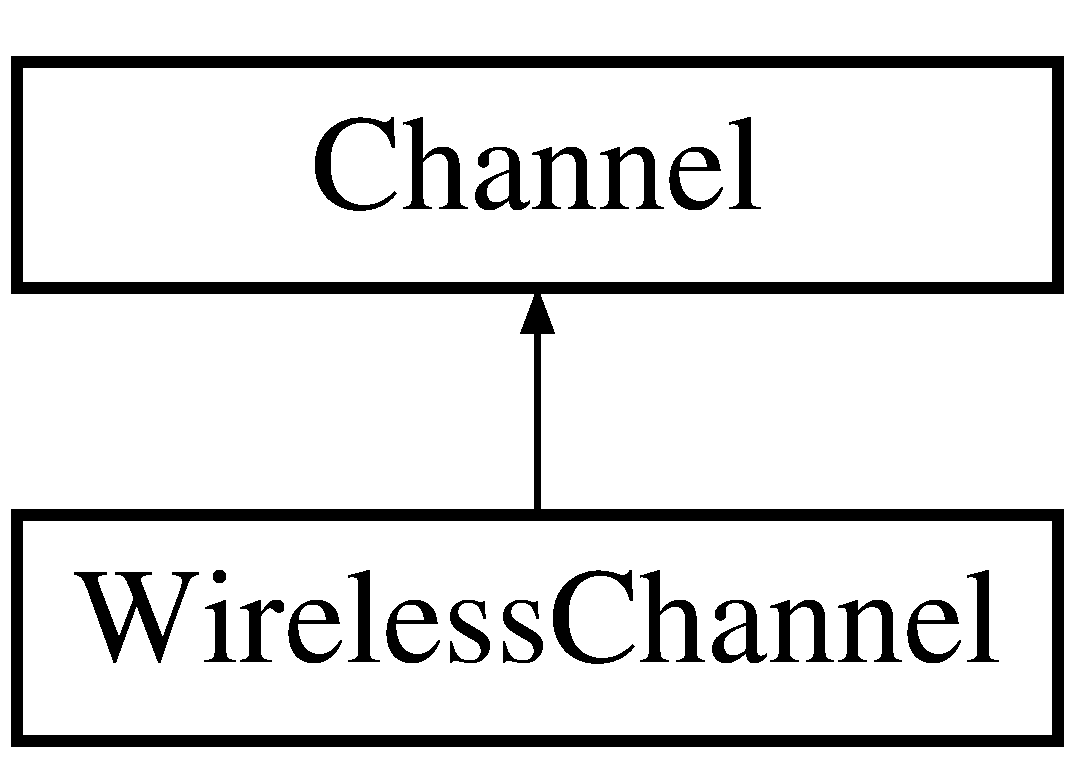
\includegraphics[height=2cm]{classChannel}
\end{center}
\end{figure}
\subsection*{Public Types}
\begin{CompactItemize}
\item 
typedef boost::shared\_\-ptr$<$ \bf{Channel} $>$ \bf{Channel\-Ptr}\label{classChannel_c81a065919781b21f07ce3ac6e354675}

\begin{CompactList}\small\item\em Smart pointer that clients should use. \item\end{CompactList}\end{CompactItemize}
\subsection*{Public Member Functions}
\begin{CompactItemize}
\item 
virtual \bf{$\sim$Channel} ()\label{classChannel_5f15ebd302464069f1a9e3f0ded14482}

\begin{CompactList}\small\item\em A destructor. \item\end{CompactList}\item 
virtual \bf{Sim\-Time} \bf{propagation\-Delay} (const \bf{Physical\-Layer} \&sender, const \bf{Physical\-Layer} \&receiver) const 
\begin{CompactList}\small\item\em Compute the propagation delay between two physical layer objects. \item\end{CompactList}\end{CompactItemize}
\subsection*{Protected Member Functions}
\begin{CompactItemize}
\item 
\bf{Channel} ()
\begin{CompactList}\small\item\em A constructor. \item\end{CompactList}\item 
\bf{Channel} (const \bf{Channel} \&rhs)
\begin{CompactList}\small\item\em A copy constructor. \item\end{CompactList}\end{CompactItemize}


\subsection{Detailed Description}
A channel class is one over which a signal travels according to some path loss model. 

In the future, this could be the superclass for sensed events as well (e.g., temperature, light), but for now it is just use for the wireless communication channel. 



Definition at line 21 of file channel.hpp.

\subsection{Constructor \& Destructor Documentation}
\index{Channel@{Channel}!Channel@{Channel}}
\index{Channel@{Channel}!Channel@{Channel}}
\subsubsection{\setlength{\rightskip}{0pt plus 5cm}Channel::Channel ()\hspace{0.3cm}{\tt  [protected]}}\label{classChannel_f2b4b16288cbb2c592b1e0f6486c2430}


A constructor. 

This is protected to ensure that all objects are created via {\tt new} since we are using smart pointers. 

Definition at line 6 of file channel.cpp.\index{Channel@{Channel}!Channel@{Channel}}
\index{Channel@{Channel}!Channel@{Channel}}
\subsubsection{\setlength{\rightskip}{0pt plus 5cm}Channel::Channel (const \bf{Channel} \& {\em rhs})\hspace{0.3cm}{\tt  [protected]}}\label{classChannel_4bee049fc3ff144e7273e29fe11a0ec4}


A copy constructor. 

This is protected to ensure that all objects are created via {\tt new} since we are using smart pointers. 

\subsection{Member Function Documentation}
\index{Channel@{Channel}!propagationDelay@{propagationDelay}}
\index{propagationDelay@{propagationDelay}!Channel@{Channel}}
\subsubsection{\setlength{\rightskip}{0pt plus 5cm}\bf{Sim\-Time} Channel::propagation\-Delay (const \bf{Physical\-Layer} \& {\em sender}, const \bf{Physical\-Layer} \& {\em receiver}) const\hspace{0.3cm}{\tt  [virtual]}}\label{classChannel_9ca936663d2dbb0236fc7df48ad23b26}


Compute the propagation delay between two physical layer objects. 

\begin{Desc}
\item[Parameters:]
\begin{description}
\item[{\em sender}]the sending physical layer. \item[{\em receiver}]the receving physical layer. \end{description}
\end{Desc}
\begin{Desc}
\item[Returns:]the propagation delay between the two objects. \end{Desc}


Definition at line 16 of file channel.cpp.

References Location::distance(), Physical\-Layer::get\-Location(), and SPEED\_\-OF\_\-LIGHT.

The documentation for this class was generated from the following files:\begin{CompactItemize}
\item 
channel.hpp\item 
channel.cpp\end{CompactItemize}
